Considere un grafo dirigido o no dirigido sin bucles ni aristas múltiples. Tenemos que comprobar si es acíclico y, si no lo es, encontrar cualquier ciclo. Considere un gráfico sucesor que solo contiene una ruta que termina en un ciclo. Nosotros podemos plantearnos las siguientes preguntas: si comenzamos nuestra caminata en el nodo inicial, ¿Cuál es el primer nodo del ciclo y cuántos nodos contiene el ciclo?

Por ejemplo, en el grafo:

% TODO: \usepackage{graphicx} required
\begin{figure}[h!]
	\centering
	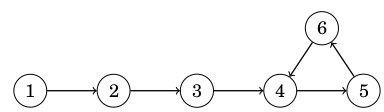
\includegraphics[width=0.7\linewidth]{img/cycle_detection}
	\label{fig:cycledetection}
\end{figure}


Si comenzamos nuestra caminata en el nodo 1, el primer nodo que pertenece al ciclo es el nodo 4,
y el ciclo consta de tres nodos (4, 5 y 6). De como detectar la existencia o no de un ciclo en grafo de acuerdo a su tipo tratará la siguiente guía.